\documentclass[11pt]{article}

\usepackage{geometry}
\geometry{a4paper, margin=2.3cm}

\usepackage{fontspec}
\usepackage{amsmath}
\usepackage{unicode-math}
% Fonts: Latin Modern (fontspec / unicode-math defaults) — reliably bundled with tectonic.

\usepackage{microtype}
\usepackage{booktabs}
\usepackage{graphicx}
\graphicspath{{./}}
\usepackage{caption}
\captionsetup{font=small, labelfont=bf}
\usepackage[dvipsnames]{xcolor}
\usepackage[colorlinks=true, linkcolor=RoyalBlue, urlcolor=RoyalBlue, citecolor=RoyalBlue]{hyperref}
\usepackage{enumitem}

\setlength{\parindent}{0pt}
\setlength{\parskip}{0.45em}
\setlist{leftmargin=1.4em}
\setlength{\emergencystretch}{3em}

\newcommand{\tp}{^{\top}}
\newcommand{\bc}{\mathbf{c}}
\newcommand{\bb}{\mathbf{b}}
\newcommand{\bG}{\mathbf{G}}
\newcommand{\bZ}{\mathbf{Z}}
\newcommand{\bA}{\mathbf{A}}
\newcommand{\bd}{\mathbf{d}}
\newcommand{\bu}{\mathbf{u}}

\title{\bfseries Exact optimum contribution selection at genomic scale:\\ a matrix-free, support-first solver validated against optiSel and AlphaMate on real marker panels}
\author{\textbf{Adel Kaleche}\\[2pt] \small\itshape Independent researcher, France.}
\date{}

\begin{document}
\maketitle

\begin{abstract}
\noindent
Optimum contribution selection (OCS) --- maximise genetic gain subject to a cap on the coancestry of the next generation --- balances gain against the loss of diversity in breeding programmes. Its bottleneck is the relationship matrix it constrains: at genomic scale that matrix is dense and $n\times n$, costing $O(n^2 m)$ to build and $O(n^2)$ to store, so the established exact (optiSel) and heuristic (AlphaMate) tools reach a memory wall as candidate numbers grow. We present \textbf{support-first}, an exact solver resting on two facts of OCS: the optimal contribution vector is supported on a small subset of candidates, and within a fixed support the kinship-constrained subproblem has a closed form. Support-first grows the support by a reduced-cost, column-generation rule and solves each fixed support in closed form, with no inner iterative solver --- which yields two distinct results. First, \emph{given} the relationship matrix, the active set exploits solution-support sparsity and reaches the exact optimum $2$--$482\times$ faster than optiSel's interior-point solve depending on the operating point ($12$--$132\times$ at $\Delta F=1\%$, the FAO floor for the rate of inbreeding), because it prices candidates in $O(n^2)$, independent of the marker count. Second, the kinship products $\bG\bc$ are formed matrix-free from the genotype matrix $\bZ$, so the solver never forms the dense $\bG$: it solves an instance ($n=40000$, $m=1000$) whose $11.9$\,GiB dense matrix will not fit. This memory advantage is the regime $m<n$ for a dense $\bZ$; storing $\bZ$ at two bits per genotype (the solver's packed path, verified to return the identical optimum) shifts the crossover to $m<32n$ and holds a national-scale panel ($n=5\times10^5$, $m=5\times10^4$) in $6.25$\,GB where the dense $\bG$ would need two terabytes. The matrix-free product costs $O(nm)$ per iteration, so it is the large-$n$ enabler, not a universal speed-up. On real panels (CIMMYT wheat, a PIC pig panel with 52k SNP, a heterogeneous-stock mouse panel with real sex) support-first returns the exact optimum on the kinship boundary, agreeing to $10^{-8}$ with a conic interior-point solver that stops just inside it; per-candidate contribution caps ($0\le\bc\le\bu$) are supported. Support-first makes exact, reproducible OCS practical at population scale.
\end{abstract}

\section{Introduction}

Genetic improvement of livestock and crops must hold two objectives in tension: maximising the genetic merit of the next generation, and conserving the genetic diversity whose erosion drives inbreeding depression and forecloses future response to selection. Optimum contribution selection (OCS; Meuwissen 1997) makes that trade-off explicit. Given each candidate's estimated breeding value and the matrix of relationships among candidates, OCS chooses the proportional genetic contributions $\bc$ that maximise expected gain $\bb\tp\bc$ subject to a cap on the mean coancestry of the offspring, $\bc\tp\bG\bc\le k$, with the contributions non-negative and summing to one --- and, in any real mating scheme, split so that sires and dams each supply half. OCS is the de facto framework for managing diversity in both commercial breeding and conservation programmes, and the genomic relationship matrix (VanRaden 2008) has largely replaced its pedigree-based predecessor as the $\bG$ it constrains.

With genomic data this is a convex quadratically constrained quadratic program, equivalently a second-order cone program, and two costs come to dominate as candidate numbers grow. The first is the relationship matrix itself: dense and $n\times n$, it costs $O(n^2)$ to store and $O(n^2 m)$ to build from $m$ markers, and at tens of thousands of candidates it no longer fits in a workstation's memory. The second is the conic solve. Yet the optimal contribution vector is almost always supported on a handful of individuals --- a sparsity that, as we show, stays bounded as $n$ grows at a fixed operating point --- and general-purpose solvers exploit neither this nor the cheap structure of the kinship constraint.

The tools in use span the exact and the heuristic, but share a template: assemble the full relationship matrix and hand the whole problem to a generic optimiser over every candidate. Meuwissen's original method (1997), and its successor Gencont2 (Dagnachew \& Meuwissen 2016), iterate the Lagrangian conditions over the full candidate set. The optiSel package (Wellmann 2019), the standard exact tool, casts OCS as a cone program for a primal-dual interior-point solver. Semidefinite formulations (Pong-Wong \& Woolliams 2007) and recent ADMM/JuMP solvers (Waldmann 2025) follow suit, the latter forming the dense $\bG$ explicitly and truncating small contributions only after the fact. AlphaMate (Gorjanc \& Hickey 2018) trades exactness for a differential-evolution heuristic that also allocates matings. The lone attempt to exploit sparsity, Yamashita, Mullin \& Safarina (2018), exploits the sparsity of the \emph{pedigree inverse} $\bA^{-1}$ --- a property of the data matrix --- inside a full-candidate interior-point solve; it is neither the sparsity of the \emph{solution} nor a genotype-based, matrix-free method. None of these exploits the two facts that make genomic OCS cheap: that the optimal support is small at a given operating point, and that within a fixed support the kinship-constrained subproblem is solvable in closed form. None avoids materialising $\bG$, which becomes the binding constraint --- in memory and in build time --- exactly at the population sizes where OCS matters.

We present \textbf{support-first}, an exact OCS solver built on those two facts. It maintains a small working support, seeded with the best candidate of each sex and grown by an active-set, reduced-cost rule: candidates are priced against the current multipliers and the one most worth adding is brought in, candidates that turn negative are dropped, all toward a single fixed coancestry cap $k$. Each fixed-support subproblem --- maximise a linear form over an ellipsoid intersected with the affine sum (and sex) constraints --- is solved in closed form by eliminating the equality constraints and reducing to a scalar quadratic in the binding multiplier, with no inner iterative solver. The kinship products $\bG\bc$ are formed matrix-free from the centred genotype matrix $\bZ$ as $\varepsilon\bc + \bZ(\bZ\tp\bc)/s$, so the solver never builds or stores the dense $n\times n$ $\bG$.

The individual ingredients are classical, and we claim none of them. Active-set methods that track a small working set of held assets descend from Markowitz's critical line algorithm (1956) for long-only mean--variance selection, of which OCS is the kinship-constrained analogue; the closed form for a linear objective over an ellipsoid intersected with linear constraints is a constrained-eigenvalue / secular-equation result (Gander, Golub \& von Matt 1989); and the matrix-free product $\bZ(\bZ\tp\bc)$ is standard in genomic prediction (VanRaden 2008; Legarra \& Misztal 2008). Our contribution is their \textbf{synthesis, specialised to genomic OCS}: reduced-cost column generation that grows a small support toward a \emph{single} coancestry cap --- as opposed to the critical line algorithm's parametric sweep of the \emph{entire} efficient frontier --- with the kinship product evaluated matrix-free, so that the cost of a solve follows the support size and the marker count rather than the dense $n\times n$ matrix. Prior OCS methods do touch solution-support sparsity, but from the other direction: Meuwissen's method (1997) solves on the full candidate set and \emph{prunes} candidates whose contribution turns negative --- a decreasing active set on the dense $n\times n$ system. Ours grows the support from below by reduced-cost column generation and never forms that system, and to our knowledge no prior OCS method combines an increasing, genotype-matrix-free active set in this way; the benefit is the combination rather than any one part.

We evaluate it on three real marker panels: a CIMMYT wheat panel ($n=599$), a PIC pig panel ($n=3534$, 52k SNP) and a heterogeneous-stock mouse panel ($n=1814$, with real sex). It reaches the exact optimum on each, agreeing with the conic optimum to $10^{-8}$. At matched realised coancestry it agrees with the interior-point methods; where they halt just inside the constraint it reaches the boundary, so its small edge there is the diversity budget they leave unspent, not a different optimum.

This yields two distinct advantages. \emph{Given} the relationship matrix, support-first's active set reaches the same optimum as optiSel's interior-point solve $2$--$482\times$ faster depending on the operating point ($12$--$132\times$ at $\Delta F=1\%$, rate of inbreeding), because it prices candidates in $O(n^2)$ regardless of the marker count --- the algorithmic gain of exploiting solution-support sparsity. Forming $\bG$ matrix-free instead trades that for never storing the $n\times n$ matrix, at $O(nm)$ per iteration; this is what lets the solver run at population sizes where $\bG$ cannot be formed, and --- because the per-iteration cost then scales with the marker count --- it is the faster route only up to moderate marker density, not on the densest panels. Against a general conic solver (Clarabel) the advantage grows with $n$ --- ${\sim}714\times$ at $n=10000$ at $\Delta F=1\%$, and ${\sim}76000\times$ at a loose cap --- in a Rust-against-Rust comparison that carries no language confound. Against AlphaMate, a heuristic for the distinct problem of discrete mate allocation, the exact optimum is no worse at matched coancestry on the continuous relaxation the two share.

The enabling result, though, is memory rather than speed. Because the solve never forms the $n\times n$ matrix, it runs where the established tools cannot: at a fixed operating point ($\Delta F=1\%$) on structured populations the support holds near 90 and the solve near 0.3\,s as $n$ grows from 1000 to 40000, while the dense $\bG$ the alternatives must materialise reaches 11.9\,GiB --- a 40$\times$ larger footprint than $\bZ$ and past the working memory of an 8--16\,GB laptop. At that size the question is no longer how fast the established tools run, but whether they run at all. Support-first makes exact, reproducible optimum contribution selection practical at population scale, on a laptop.

\section{Methods}

\subsection{Optimum contribution selection}

For $n$ selection candidates with estimated breeding values $\bb\in\mathbb{R}^n$ and a genomic relationship matrix $\bG\in\mathbb{R}^{n\times n}$, optimum contribution selection chooses proportional genetic contributions $\bc$ that solve
\[
  \text{maximise } \bb\tp\bc \quad\text{subject to}\quad \bA\bc=\bd,\ \ 0\le\bc\le\bu,\ \ \bc\tp\bG\bc\le k.
\]
The affine constraints $\bA\bc=\bd$ encode the contribution budget. In the simplex form a single row $\bA=\mathbf{1}\tp$, $\bd=1$, imposes $\sum_i c_i = 1$. In the \emph{sexed} form --- the true OCS, since each mating draws one parent of each sex --- $\bA$ is the $2\times n$ sex-incidence matrix (row 1 the male indicator, row 2 the female indicator) and $\bd=(\tfrac12,\tfrac12)\tp$, imposing $\sum_{\text{males}} c_i = \sum_{\text{females}} c_i = \tfrac12$. The per-candidate cap $\bu$ bounds any single individual's contribution --- a breeder rarely lets one parent dominate a generation --- and is inactive at $\bu=1$. The kinship bound $\bc\tp\bG\bc\le k$ caps the mean coancestry of the offspring. We index operating points by the effective number of contributing parents $N_e=1/\sum_i c_i^2$, with the rate of inbreeding $\Delta F\approx1/(2N_e)$ (Woolliams \& Bijma 2000), and select the cap $k$ that attains a target $N_e$ by bisection --- so a ``$\Delta F=1\%$'' row is the cap giving $N_e=50$. This $N_e$ is a genomic contribution-variance quantity, a defensible but not identical proxy for the demographic $N_e$ the FAO floor ($N_e\ge50$) refers to. We take $\bG$ as the VanRaden genomic relationship matrix, $\bG=\bZ\bZ\tp/s+\varepsilon\mathbf{I}$, where $\bZ$ is the $n\times m$ matrix of genotypes centred by twice the allele frequencies, $s=2\sum_j p_j(1-p_j)$, and $\varepsilon$ a small ridge ensuring positive definiteness (the same ridged matrix the conic baselines constrain, so all solvers face an identical problem). The program is a convex quadratically constrained quadratic program, equivalently a second-order cone program.

\subsection{Two structural facts}

Support-first rests on two properties of the optimum $\bc^*$. First, at a binding kinship cap $\bc^*$ is supported on a small set $S=\{i: 0<c^*_i<u_i\}$ of \emph{free} contributions, and $S$ is empirically bounded as $n$ grows at a fixed operating point (Results). Second, on the face where the inactive bound constraints are dropped (candidates fixed at 0 or at their cap $\bu$), the problem restricted to $S$ --- maximise a linear form over an ellipsoid intersected with the affine constraints --- has a closed-form solution. The whole difficulty is therefore identifying $S$ and which candidates sit at their cap; everything else is a small direct solve.

\subsection{Closed form on a fixed support}

Fix a support $S$ of size $|S|$, and write $\bG_S$, $\bb_S$, $\bA_S$ for the restrictions to $S$ ($\bA_S$ is $q\times|S|$ with $q=1$ or 2 equality rows). At the optimum of the restricted problem the kinship constraint is active, and the stationarity conditions read
\[
  \bb_S = \bA_S\tp\mu + 2\lambda\,\bG_S\bc_S,\qquad \bA_S\bc_S=\bd,\qquad \bc_S\tp\bG_S\bc_S=k,
\]
with multipliers $\mu\in\mathbb{R}^q$ and $\lambda\ge0$. Solving stationarity for $\bc_S$ gives $\bc_S=\tfrac{1}{2\lambda}\bG_S^{-1}(\bb_S-\bA_S\tp\mu)$. Imposing the affine constraints eliminates $\mu$: with the $q\times q$ matrix $\mathbf{P}=\bA_S\bG_S^{-1}\bA_S\tp$ and vector $\mathbf{q}_v=\bA_S\bG_S^{-1}\bb_S$,
\[
  \mu=\mathbf{P}^{-1}(\mathbf{q}_v-2\lambda\bd),\qquad\text{so}\qquad \bc_S=\mathbf{g}/(2\lambda)+\mathbf{h},
\]
where $\mathbf{g}=\bG_S^{-1}(\bb_S-\bA_S\tp\mathbf{P}^{-1}\mathbf{q}_v)$ and $\mathbf{h}=\bG_S^{-1}\bA_S\tp\mathbf{P}^{-1}\bd$ satisfy $\bA_S\mathbf{g}=\mathbf{0}$ and $\bA_S\mathbf{h}=\bd$, so $\bA_S\bc_S=\bd$ for every $\lambda$. Substituting into the active ellipsoid $\bc_S\tp\bG_S\bc_S=k$ and writing $\alpha=\mathbf{g}\tp\bG_S\mathbf{g}$, $\beta=\mathbf{g}\tp\bG_S\mathbf{h}$, $\gamma=\mathbf{h}\tp\bG_S\mathbf{h}$ yields a single scalar quadratic in the multiplier:
\[
  4(\gamma-k)\,\lambda^2 + 4\beta\,\lambda + \alpha = 0.
\]
We take the positive root maximising $\bb_S\tp\bc_S$. Because $\bG_S\mathbf{g}=\bb_S-\bA_S\tp\mathbf{P}^{-1}\mathbf{q}_v$ and $\bG_S\mathbf{h}=\bA_S\tp\mathbf{P}^{-1}\bd$ are already available, $\alpha,\beta,\gamma$ cost only inner products --- no second factorisation. A restricted solve is thus: one Cholesky factorisation of $\bG_S$, back-substitutions for the $q+1$ right-hand sides $[\bA_S\tp\mid\bb_S]$, a $q\times q$ inverse ($q\le2$), and a scalar quadratic --- no inner iteration. The simplex case ($q=1$, $\bA_S=\mathbf{1}\tp$) is identical and reduces to a scalar quadratic in $\mu$. When the equalities fully determine $\bc_S$ ($|S|=q+1$) the contributions are forced --- $(\tfrac12,\tfrac12)$ in the sexed case --- and we set $\lambda=0$ (the binding subcase is measure-zero, as for a singleton support). The solve returns ``infeasible on $S$'' when $S$ lacks a sex or the ellipsoid does not meet the affine hull, the signal to enlarge $S$.

\subsection{The support-first algorithm}

The support is found by active-set column generation. It is seeded with the best candidate of each sex, $S=\{\arg\max_{\text{males}} b,\ \arg\max_{\text{females}} b\}$. Each iteration solves the closed form on the current $S$ and branches:

\begin{itemize}
\item \textbf{Infeasible on $S$} (the support is too related to meet the cap $k$): add the least-related candidates, those with the smallest $(\bG\bc)_j$, in a chunk that doubles $|S|$. This feasibility phase, when done one candidate at a time, was the dominant cost; chunking cut total iterations roughly thirty-fold with an identical optimum.
\item \textbf{A contribution is negative}: drop every $i$ with $c_{S,i}\le0$, marking them taboo to re-entry until the next genuine improvement, and re-solve; if dropping empties a sex, its best candidate is re-seeded.
\item \textbf{Otherwise}: price each candidate $j\notin S$ by its reduced cost $r_j=b_j-\mu_{\text{sex}(j)}-2\lambda(\bG\bc)_j$, and add the maximiser if $r_j>\text{tol}$; if none is positive, stop. A genuine addition clears the taboo set.
\end{itemize}

Because the problem is convex, a feasible point at which no candidate has a positive reduced cost satisfies the Karush--Kuhn--Tucker conditions and is the global optimum; correctness is therefore not heuristic. The taboo set together with a degeneracy threshold scaled to the coefficient magnitudes prevented cycling on every instance solved here, though we do not prove finite termination in general. The closed form stays well-conditioned in practice: with the ridge $\varepsilon$, $\kappa(\bG_S)$ ran from about 10 to 4000 at operating supports on the real panels (highest on the autogamous wheat lines), and a block of exact-duplicate genotypes --- a singular $\bG_S$ absent the ridge --- still solved to a feasible KKT optimum, the duplicates splitting their contribution evenly. Reduced-cost pricing toward a \emph{single} fixed cap $k$ distinguishes the support update from the critical line algorithm, which changes the active set by $\pm1$ along a swept multiplier to trace the whole efficient frontier.

A per-candidate cap $\bc\le\bu$ is absorbed by the same active set with no loss of the closed form. A free contribution that overshoots its cap is fixed at $u_j$ and moved to an \emph{upper} set $U$; a candidate already in $U$ is released back to the free set when its reduced cost turns negative. With $U$ fixed, the restricted solve keeps its structure --- the fixed contributions enter the affine right-hand side as $\bd-\bA_U\bu_U$ and the active ellipsoid as a matrix-free offset $\bG_{\cdot U}\bu_U$ plus a constant, leaving the same Cholesky and scalar quadratic. The bounded solve reduces to the unbounded one when no cap binds, and reaches the same optimum as a conic interior-point solver on the matching $\bc\le\bu$ cone program under binding caps.

\subsection{Matrix-free kinship products}

Every full kinship product is formed without materialising $\bG$:
\[
  \bG\bc = \varepsilon\,\bc + \bZ(\bZ\tp\bc)/s,
\]
two matrix--vector products against the $n\times m$ genotype matrix, at $O(n\cdot m)$ time and $O(n\cdot m)$ memory for $\bZ$ versus $O(n^2)$ for a dense $\bG$. The restricted $\bG_S$ is assembled only on the support. $\bZ$ is held at two bits per genotype (the three dosages need no more), centring applied on the fly through rank-1 corrections, so its footprint is $nm/4$ bytes --- a further $32\times$ below a dense-$f64$ $\bZ$; the packed and dense solves are verified to return the same optimum to machine precision. This is the enabler at large $n$, where the dense $n\times n$ $\bG$ is infeasible to store or costly ($O(n^2 m)$) to build; it is not an inner-loop speed-up when $m>n$, and the advantage over the conic baselines is algorithmic --- the small active set --- independent of this choice.

\subsection{Implementation and reproducibility}

The solver is implemented in Rust over a pure-Rust stack: dense linear algebra (the support Cholesky and back-substitutions) via \texttt{faer}, with no system BLAS/LAPACK dependency, no \texttt{unsafe}, and a seeded reproducible RNG for the synthetic generators. A conic interior-point solver (\texttt{clarabel}) is included only as an independent oracle for cross-checking. Correctness is asserted by KKT-certificate unit tests across a range of caps $k$ --- a \texttt{Solved} result is always feasible, on the budget, and sex-split --- and by cross-language agreement: on a binding instance the Rust \texttt{solve\_sexed} reproduces a NumPy reference optimum to a gain difference of $1.5\times10^{-14}$. The build is gated on \texttt{cargo fmt}, \texttt{cargo clippy -D warnings}, and the test suite.

\subsection{Data and baselines}

The method is evaluated on three public marker panels: a CIMMYT wheat panel (\texttt{BGLR}, $n=599$), a PIC pig panel ($n=3534$, 52k SNP, with real estimated breeding values), and a heterogeneous-stock mouse panel (\texttt{BGLR}, $n=1814$, with recorded sex, 934 males and 880 females, using body-mass index as the selection criterion). For each, $\bG$ is the VanRaden matrix with ridge $\varepsilon=10^{-5}$.

A fourth instance is derived from the PIC panel and is the only one carrying a real breeding value and a real sex at once. The PIC download ships a pedigree, and a pedigree assigns sex without ambiguity: an animal appearing in the sire column is male, in the dam column female. Intersecting that with the genotyped animals recovers a recorded sex for 1194 of the 3534 (390 sires, 804 dams; no animal appears as both), each of which carries a real estimated breeding value from the accompanying evaluation (mean accuracy 0.811 on trait 3). Allele frequencies, and hence $\bG$, are recomputed on the retained animals. Because sex is recoverable here precisely for the animals that became parents, this sub-panel is a post-selection subset rather than a random sample of selection candidates --- a property of the recovery, not a choice, and one that bears on the interpretation of the contribution vector rather than on what the benchmark measures. Because the values that panel ships come from the breeding programme's own evaluation and are not genomic predictions, the sub-panel is also run with a criterion computed the way genomic selection computes it: a GBLUP fitted by \texttt{BGLR} on the panel's own trait-3 phenotypes (3141 of the 3534 animals) against its own genomic relationship matrix, with the criterion read back as the posterior mean of the genetic effect. The fitted genomic heritability is 0.247, and 119 of the 1194 sub-panel animals carry no phenotype of their own, so their value comes entirely from genomic relationships --- the case genomic selection exists for.

Baselines are optiSel (R, the \texttt{cccp} Nesterov--Todd interior-point solver; the exact domain reference), Clarabel (the conic cross-check), and AlphaMate (Fortran differential evolution; run from its Linux binary under emulation, as no macOS build exists and the source is locked to an Intel toolchain). Caveats carried into the Discussion: recorded sex is real for the mouse panel and for the sexed pig sub-panel, while wheat (autogamous) and the full pig panel use an arbitrary balanced split; the selection criterion $\bb$ is a real estimated breeding value on the pig panels and a recorded phenotype standing in for one on wheat and mouse; and Table~\ref{tab:optisel} reports two support-first timings against optiSel --- the active set given a dense $\bG$ (the regime optiSel runs in, a NumPy prototype) and the shipped matrix-free Rust solver end to end --- so the algorithmic advantage and what the shipped tool actually pays are separated rather than conflated. The Clarabel comparison (Table~\ref{tab:clarabel}) is Rust against Rust in one process, and so carries no language confound at all.

\section{Results}

\subsection{Exactness}

Support-first is exact by construction: for a convex program a feasible point at which no candidate has a positive reduced cost satisfies the KKT conditions, and this is what the active set certifies on termination (and what the unit tests assert across a range of kinship caps). Empirically, on the optiSel \texttt{Cattle} example (Angler cattle, $n=268$) using the sex the package ships (its phenotypes are simulated, which does not matter here: this is a solver-against-solver agreement check, not a claim about cattle), support-first and optiSel select the \emph{same} 36-individual support and agree on the contributions to within $3\times10^{-4}$ (maximum contribution 0.0664 vs 0.0661). They differ only at the kinship boundary: the OCS optimum sits on the cap (gain is monotone in it), and support-first reaches it ($\bc\tp\bG\bc=k$), whereas optiSel's interior-point solver halts at its convergence tolerance just inside the feasible region (group kinship 0.0576 against a bound of 0.0578). At operating caps support-first reaches the boundary while optiSel's interior-point solver halts progressively further inside it as the cap tightens --- on the mouse panel optiSel reaches $98.2\%$, $95.3\%$ and $85.7\%$ of the cap at $\Delta F=2/1/0.5\%$ (support 47/89/182) against support-first's $100\%$, the gain gap growing from $3\times10^{-4}$ to $2.6\times10^{-3}$. Support-first's edge is thus the diversity budget optiSel leaves unspent --- more pronounced at the tighter, operationally relevant caps --- not a different optimum: the difference is boundary-saturation versus an interior stop. Against an independent conic interior-point solver (Clarabel) on synthetic data the two agree to a gain difference below $10^{-8}$ across kinship caps, and the Rust implementation of the sexed solver reproduces a NumPy reference optimum to $1.5\times10^{-14}$ on a binding instance. Support-first is therefore at least as accurate as the domain tool, and exact where the interior-point methods are merely close. The per-candidate-capped form ($0\le\bc\le\bu$) advertised in the abstract is exercised, not merely declared: on the matching $\bc\le\bu$ cone program the capped solve reproduces Clarabel's optimum (unit-tested), the bounds entering the same closed form as an upper-set offset.

\subsection{Speed against a generic conic solver}

This comparison also settles a question the optiSel head-to-head cannot: both solvers here are Rust, called in the same process on the same generated data, so no language difference can be mistaken for an algorithmic one. On synthetic genomic instances at a breeder operating point ($\Delta F\approx1\%$, support ${\approx}100$) support-first's advantage over the Clarabel conic solver grows steeply with $n$ (Table~\ref{tab:clarabel}): from parity at $n=1000$ to ${\sim}714\times$ at $n=10000$, where the conic route takes 38 minutes and support-first 3.2\,s. The scaling is structural --- Clarabel factors a dense $O(n^3)$ KKT system at every interior-point iteration (2.1\,s to 2290\,s across the sweep), whereas support-first performs ${\sim}150$--$170$ matrix--vector products, each $O(n\cdot m)$, its time growing only gently (1.4\,s to 3.2\,s). At a loose cap the support collapses to a handful and the factor reaches ${\sim}76000\times$; that is the easy end, and we report the operating point instead.

\begin{table}[ht]
\centering
\caption{support-first vs Clarabel at a breeder operating point, identical optimum (agreeing to ${\sim}10^{-8}$ in gain), one serial sweep on an idle machine. Both solvers are Rust in one process on the same synthetic instance ($m=20000$, cap tuned to a support of ${\approx}100$, i.e.\ $\Delta F\approx1\%$), so the comparison carries no language confound.}
\label{tab:clarabel}
\begin{tabular}{rrrrr}
\toprule
$n$ & $m$ & Clarabel\textsuperscript{1} & support-first & speed-up \\
\midrule
1000  & 20000 & 2.22\,s   & 1.43\,s & 1$\times$ \\
2000  & 20000 & 16.2\,s   & 1.90\,s & 9$\times$ \\
5000  & 20000 & 308\,s    & 2.36\,s & 131$\times$ \\
10000 & 20000 & 2298\,s   & 3.21\,s & \textbf{716$\times$} \\
\bottomrule
\end{tabular}
\end{table}

\noindent\textsuperscript{1}\,the whole conic route: forming $\bG$, its Cholesky, cone assembly and the interior-point solve. The interior-point solve alone is 2.1\,/\,15.9\,/\,306\,/\,2290\,s. support-first's column is its entire run, since it builds nothing.

Two qualifications. The large-$n$ cells are single runs (Clarabel needs 38 minutes at $n=10000$); the support-first side is deterministic. And the advantage is entirely $n$-driven: at $n=1000$ the two are at parity, because at $m=20000$ support-first's ${\sim}150$ products at $O(nm)$ match Clarabel's $O(n^3)$ solve at small $n$ --- the gap opens only as $n^3$ overtakes $n\cdot m$.

\subsection{Speed against the domain tool optiSel}

A generic solver is a soft target; the informative comparison is against optiSel, the standard exact OCS tool, on its own formulation. After extending support-first to the two sex-equality constraints it returns the same optimum as optiSel throughout. We measure at breeder-relevant operating points --- a target rate of inbreeding $\Delta F$, equivalently an effective number of parents $N_e\approx1/(2\Delta F)$ --- rather than at a loose cap, and we separate two things an earlier version of this comparison conflated: the \emph{algorithm} (the active set given the relationship matrix, as the interior-point tools have it) and the \emph{matrix-free representation} (the shipped solver, which forms no $\bG$). Table~\ref{tab:optisel} reports both at $\Delta F=1\%$ ($N_e=50$, the FAO floor). Given $\bG$, the active set reaches optiSel's optimum $12$--$132\times$ faster on every panel, because it prices candidates in $O(n^2)$ --- independent of the marker count $m$. The matrix-free solver instead pays $O(nm)$ per iteration, so its end-to-end speed-up follows the marker density: $3\times$ on wheat, ${\sim}6\times$ on mouse, but on the pig, with 52k markers, it is \emph{slower} than optiSel ($0.3\times$), because re-deriving kinship from $\bZ$ every iteration costs more than reusing a $\bG$ formed once at this small $n$. The two columns bracket the trade-off: the algorithmic advantage is real and $m$-independent, while the matrix-free route buys the ability to run at $n$ where $\bG$ cannot be formed (see Scaling) at the price of an $m$-dependent per-iteration cost.

\begin{table}[ht]
\centering
\caption{support-first vs optiSel at a breeder operating point ($\Delta F=1\%$, i.e.\ $N_e=50$, the FAO floor), same optimum throughout, medians on one idle machine (Apple M4 Max; R linked against OpenBLAS 0.3.33, a multithreaded BLAS, so the baseline is not a slow reference build). Two support-first columns: \emph{algorithm} = the active set given a dense $\bG$, as the interior-point tools have it, so pricing is $O(n^2)$; \emph{matrix-free} = the shipped solver, forming no $\bG$, $O(nm)$ per iteration, timed end to end from genotypes. optiSel constrains $\bc\tp\!\operatorname{sKin}\bc\le \mathrm{ub}$ on $\operatorname{sKin}=\bG/2+10^{-5}\mathbf{I}$, so support-first is handed the identical problem. The matrix-free speed-up follows the marker count $m$; the algorithmic one does not. Active-set iterations are 91/120/124 (wheat/mouse/pig); timings are medians of 3 runs for the algorithm and optiSel columns, a single timed run after warm-up for the matrix-free column.}
\label{tab:optisel}
\small\setlength{\tabcolsep}{4pt}
\begin{tabular}{lrrrrrrrr}
\toprule
dataset & $n$ & $m$ & $|S|$ & algorithm\textsuperscript{1} & matrix-free\textsuperscript{2} & optiSel & algo.\textsuperscript{3} & m-free\textsuperscript{3} \\
\midrule
CIMMYT wheat (real GRM)             & 599  & 1279  & 109 & 0.055\,s & 0.214\,s & 0.667\,s & 12$\times$ & 3$\times$ \\
HS mouse (real GRM, real sex)       & 1814 & 10346 & 89  & 0.061\,s & 1.46\,s  & 8.06\,s  & \textbf{132$\times$} & 6$\times$ \\
PIC pig, sexed (real EBV \& sex)\textsuperscript{4} & 1194 & 52843 & 110 & 0.078\,s & 10.06\,s & 2.77\,s & 36$\times$ & \textbf{0.3$\times$} \\
\bottomrule
\end{tabular}
\end{table}

\noindent\textsuperscript{1}\,active set given a precomputed dense $\bG$, solve only (NumPy prototype, so an upper bound on a Rust implementation of the same algorithm); \textsuperscript{2}\,matrix-free, forming no $\bG$, end to end from genotypes (shipped Rust); \textsuperscript{3}\,speed-up over optiSel, reported for each of the two columns; \textsuperscript{4}\,the PIC sub-panel carrying a real EBV \emph{and} a real sex (Methods).

The operating point sets the scale. At $\Delta F=2\%$ ($N_e=25$) the supports are smaller (47--57) and both routes faster --- matrix-free $9\times$ (wheat) to $34\times$ (mouse), the algorithm $40$--$482\times$; at $\Delta F=0.5\%$ ($N_e=100$) the supports run to 182--226 and the matrix-free route reaches parity or worse (mouse $0.9\times$, pig $18\times$ slower), while the algorithm stays $2$--$20\times$ ahead. The loose cap an earlier version of this work reported puts the operating point at $N_e\approx10$ ($\Delta F\approx5\%$), well below any breeding programme; the speed-ups there are larger but not the ones that matter. Across all three points the algorithm --- given $\bG$, pricing in $O(n^2)$ --- is faster than the matrix-free column on every panel, since with $m>n$ on each, $O(n^2)<O(nm)$; the matrix-free column is what it costs to keep nothing dense in memory. Both routes return the same optimum on every row, reaching the boundary optiSel stops just inside.

The pig sexed sub-panel is the one instance carrying a real breeding value \emph{and} a real sex at once, and so the closest here to what a breeding programme runs. Sex is not assumed but read off the pedigree the PIC download ships --- sire $\Rightarrow$ male, dam $\Rightarrow$ female --- resolving 1194 of the 3534 genotyped animals (390 sires, 804 dams, none appearing as both), each carrying a real EBV from the accompanying evaluation at mean accuracy 0.811. It is also the least favourable row for the matrix-free route ($m/n\approx44$), which is exactly why it is informative: it shows the matrix-free penalty at its worst \emph{and} the algorithmic advantage surviving it --- $36\times$ over optiSel given $\bG$, against the matrix-free $0.3\times$. Both routes reach the same optimum, on the boundary optiSel stops just inside, selecting 49 males and 61 females at $\Delta F=1\%$ (support 110). Repeating the comparison with a genuine GEBV --- a GBLUP fitted on the panel's own phenotypes and relationship matrix, correlating 0.64 with the shipped EBV --- changes nothing material, so the behaviour does not turn on which breeding value serves as the criterion. Caveats to the Discussion: on wheat and mouse the criterion is a recorded phenotype rather than a breeding value, and in no panel a \emph{genomic} one; and the sexed pig sub-panel, being the animals that became parents, is a post-selection subset.

\subsection{Comparison with the heuristic AlphaMate}

AlphaMate optimises a related but distinct problem --- discrete mate allocation by a stochastic evolutionary algorithm --- so this is not a like-for-like contest. We score \emph{its} contribution vector in our metric and compare, at matched group coancestry, only on the continuous-contribution relaxation the two methods share. On that relaxation support-first's exact optimum has higher gain than AlphaMate's vector at every point of its frontier (Table~\ref{tab:alphamate}): a small margin at the $45^\circ$ trade-off ($\Delta$gain $+0.004$) and larger ones at the corners --- as an exact convex optimum should against a stochastic heuristic that additionally carries integer mating constraints. This is a consistency check that support-first is exact on the shared relaxation, not a claim that AlphaMate is beaten at its own task, discrete mate allocation, which support-first does not do. AlphaMate was also markedly fragile on real genomic data: a successful run required six configurations and three work-arounds --- capping matings below $n$; restoring the full parent set, to avoid a setup segmentation fault the reduced parent count triggered; and positively shifting the criterion, to undo a sign inversion on the centred, negative EBVs --- whereas support-first and optiSel ran unmodified. We do not quote an AlphaMate run time: the only binary that ran here was an x86 build under emulation, so its wall time is not comparable.

\begin{table}[ht]
\centering
\caption{Genetic gain at matched group coancestry $\bc\tp\mathbf{K}\bc$, where $\mathbf{K}=\bG/2$ is the coancestry matrix, mouse panel; each method's contribution vector scored in the same metric.}
\label{tab:alphamate}
\begin{tabular}{lrrr}
\toprule
group coancestry $\bc\tp\mathbf{K}\bc$ & AlphaMate & support-first & $\Delta$gain \\
\midrule
0.000272 (AlphaMate min-coancestry) & $-0.45885$ & $\mathbf{-0.37843}$ & $+0.080$ \\
0.001317 (AlphaMate 45$^\circ$ optimum) & $-0.35748$ & $\mathbf{-0.35318}$ & $+0.004$ \\
0.007574 (AlphaMate max-criterion) & $-0.34066$ & $\mathbf{-0.32240}$ & $+0.018$ \\
\bottomrule
\end{tabular}
\end{table}

\subsection{Scaling and the matrix-free advantage}

The enabling advantage is memory, and unlike the speed-up it holds at every operating point. Sweeping the candidate count from 1000 to 40000 at a fixed marker panel ($m=1000$), the dense relationship matrix every other solver must materialise sets the ceiling. Merely \emph{building} it costs $O(n^2 m)$: 3.4\,s at $n=30000$, already 113$\times$ the entire matrix-free solve at that size, and rising quadratically. \emph{Storing} it costs $O(n^2)$: 11.9\,GiB at $n=40000$, where the matrix-free $\bZ$ footprint is 0.30\,GiB and the dense matrix no longer fits in a laptop's working memory (Figure~\ref{fig:scaling}B). At that size the question is not how fast the dense-$\bG$ tools run but whether they run at all. The matrix-free solve meanwhile stays cheap with its support bounded as $n$ grows \emph{at a fixed operating point}: on structured panels at $\Delta F=1\%$ the support holds near 90 and the solve near 0.3\,s to $n=40000$ (Figure~\ref{fig:scaling}A). A fixed \emph{absolute} cap would instead make the support look flat only by relaxing as the minimum achievable coancestry falls with $n$ (see \emph{Support behaviour}), which is why the figure fixes the operating point.

\begin{figure}[ht]
\centering
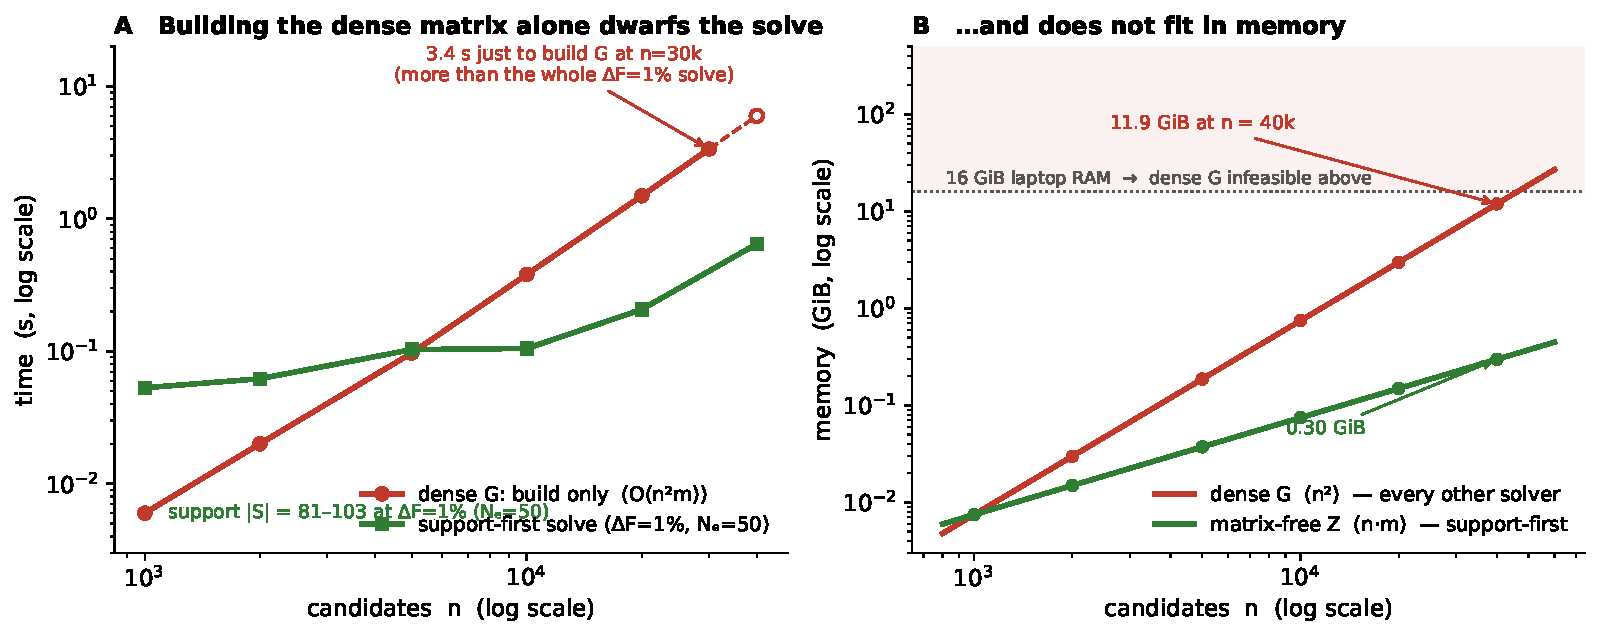
\includegraphics[width=\linewidth]{fig_scaling.pdf}
\caption{Matrix-free vs dense-$\bG$ scaling at a breeder operating point ($\Delta F=1\%$, $N_e=50$). \textbf{(A)} Building the dense $\bG$ alone ($O(n^2 m)$) rises past the whole support-first solve, whose support stays bounded (${\sim}80$--103) and time near 0.3\,s as $n$ grows to 40000. \textbf{(B)} Memory: the dense $\bG$ reaches 11.9\,GiB at $n=40000$ versus 0.30\,GiB for the matrix-free $\bZ$. The build and memory curves are operating-point-independent.}
\label{fig:scaling}
\end{figure}

\subsection{Support behaviour}

The advantage rests on the support, whose size is set by the operating point --- the target rate of inbreeding $\Delta F$, equivalently the effective number of parents $N_e\approx1/(2\Delta F)$ --- not by a universal constant, so we anchor it to the caps breeding programmes actually use rather than to a favourable one. Programmes run at $\Delta F$ of roughly $0.5$--$2\%$; the FAO floor is $N_e\ge50$, i.e. $\Delta F\le1\%$. At those caps the support on the panels here is tens to a couple of hundred, not single digits: on the mouse panel it is 47 candidates of 1814 at $\Delta F=2\%$, 89 at $1\%$ and 182 at $0.5\%$ (a loose cap, by contrast, collapses it to two, and $N_e\approx10$). Two behaviours must be kept separate. \emph{Along} the frontier the support grows as diversity is pushed --- on mouse, 47/89/182 at $\Delta F=2/1/0.5\%$, rising to ${\sim}1163$ as the cap approaches minimum coancestry. \emph{Across} population size at a fixed operating point it stays bounded: on structured (AlphaSimR) panels at $\Delta F=1\%$ the support holds near 90 as $n$ grows from 1000 to 40000, while the dense $\bG$ grows to 11.9\,GiB. A fixed \emph{absolute} cap, by contrast, only makes the support look flat as $n$ grows because the minimum achievable coancestry falls as ${\sim}1/n$ and so relaxes the constraint --- which is why we fix the operating point, not the cap. Whether the support is bounded independently of the operating point is open; the genetics supplies the growth half ($\Delta F\propto\sum c_i^2$), and the Discussion takes up the rest. Figure~\ref{fig:frontier} shows both on the real panels: the support along $\Delta F$ (A) and the matrix-free solve time (B), the latter ordered by marker count.

\begin{figure}[ht]
\centering
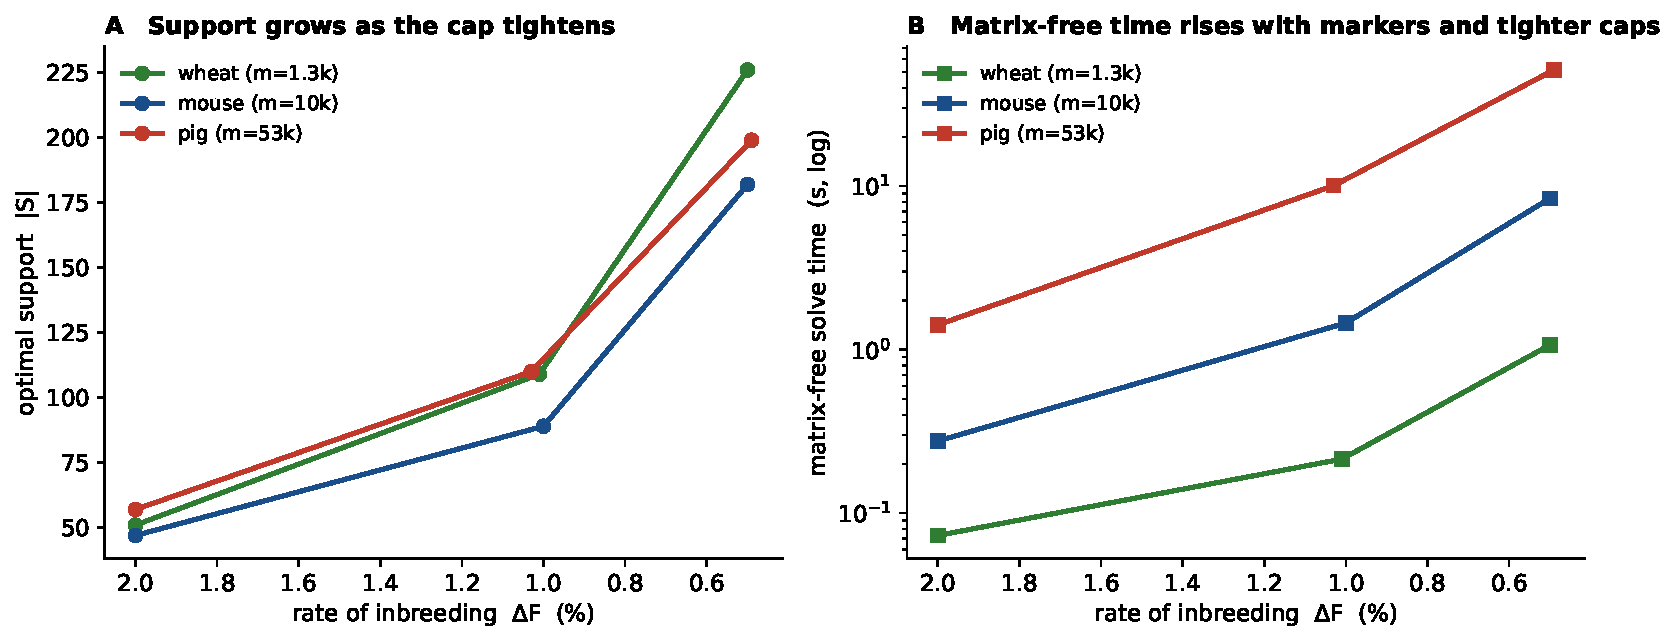
\includegraphics[width=\linewidth]{fig_frontier.pdf}
\caption{The operating-point frontier on the three real panels. \textbf{(A)} The optimal support grows as the coancestry cap tightens (smaller $\Delta F$, larger $N_e\approx1/(2\Delta F)$). \textbf{(B)} The matrix-free solve time rises with the cap and, at fixed $\Delta F$, with the marker count $m$ --- pig (53k SNP) above mouse (10k) above wheat (1.3k) --- the $O(nm)$ per-iteration cost made visible.}
\label{fig:frontier}
\end{figure}

\subsection{Multi-generation validation}

The single-generation results establish exactness and cost; the breeding question is whether recurrent support-first OCS behaves as optimum contribution selection should over generations. We ran 12 generations of recurrent selection on AlphaSimR populations (120 coalescent founders, an additive trait, 3 replicates), each generation calling the shipped R binding to solve OCS at $\Delta F=1\%$ ($N_e=50$) on the current genotypes and mating in proportion to the returned contributions, against truncation selection (top 25 of each sex by true genetic value) as the diversity-agnostic baseline. Support-first OCS retains markedly more diversity --- observed heterozygosity falls to 0.246 by generation 12 against truncation's 0.221 (both from 0.290), a ${\sim}40\%$ slower loss --- while \emph{sustaining} gain: it matches truncation early and edges ahead late (11.9 vs 11.6 at generation 12, Figure~\ref{fig:multigen}), because holding the rate of inbreeding down preserves the genetic variance that long-term response feeds on. This is the textbook case for OCS, reproduced with support-first driving every generation.

\begin{figure}[ht]
\centering
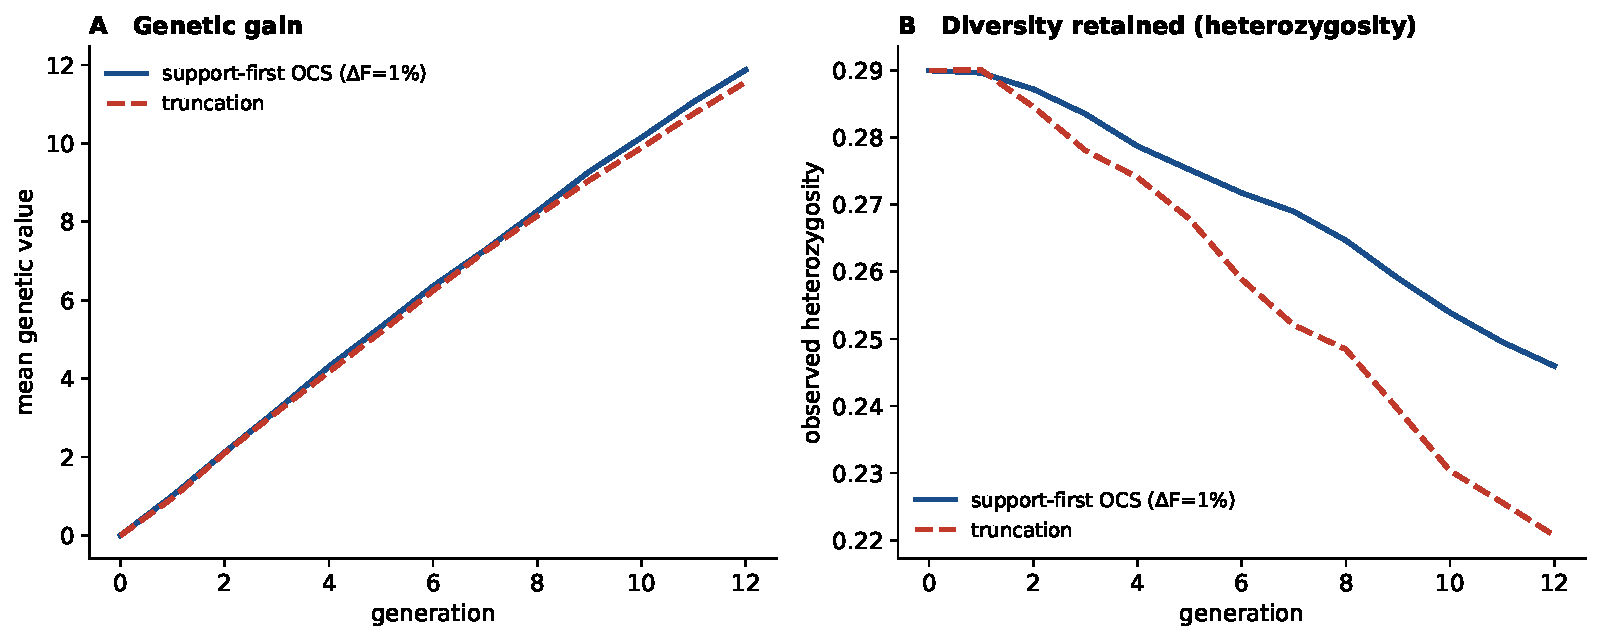
\includegraphics[width=\linewidth]{fig_multigen.pdf}
\caption{Twelve generations of recurrent selection on AlphaSimR populations (3 replicates): support-first OCS at $\Delta F=1\%$ against truncation. \textbf{(A)} Genetic gain --- OCS matches truncation and edges ahead late. \textbf{(B)} Observed heterozygosity --- OCS retains it markedly better (0.246 vs 0.221 at generation 12), the preserved variance sustaining the gain in (A).}
\label{fig:multigen}
\end{figure}

\section{Discussion}

Support-first makes exact optimum contribution selection cheap at genomic scale, in two distinct senses. Given the relationship matrix, its active set reaches the same optimum as optiSel's interior-point solve one to two orders of magnitude faster at breeder-relevant caps ($12$--$132\times$ here), by exploiting solution-support sparsity at $O(n^2)$ pricing. And by forming the kinship products matrix-free it never stores the dense matrix, so it stays runnable precisely where that matrix becomes infeasible --- the large-candidate regime that motivates genomic OCS. The matrix-free route is the enabler, not a universal speed-up: its $O(nm)$ per-iteration cost makes it slower than reusing a precomputed $\bG$ when markers greatly outnumber candidates, as on the pig. Because the method is exact and deterministic --- a Karush--Kuhn--Tucker--certified active set rather than a stochastic search --- its output is reproducible to the last digit, unlike the heuristic mate-selection tools it is measured against.

The method's ingredients are individually classical, and we claim only their synthesis. Active-set tracking of a small working set descends from the critical line algorithm for long-only mean--variance selection; the per-support closed form is a constrained-eigenvalue result; the matrix-free product is standard in genomic prediction. The contribution is their combination, specialised to OCS: reduced-cost column generation that grows a small support toward a single coancestry cap, with the kinship product evaluated matrix-free so that cost follows the support and the marker count rather than the $n\times n$ matrix. Framed against the closest prior work, this is neither the pedigree-matrix sparsity of an interior-point OCS solver nor the full-population dense solves of the standard tools. Two closer comparisons we did not run, and flag rather than dismiss. Gencont2 (Dagnachew \& Meuwissen 2016) is a Newton--Raphson on the Lagrangian conditions at $O(n^2)$ per iteration --- the same per-iteration cost as our pricing --- so at matched cost it is the fair test of whether an increasing active set converges in fewer iterations than a full-set Newton solve; its distribution is tied to pedigree relationships and we did not reimplement it on a genomic $\bG$, which is the most informative benchmark left open. Waldmann's (2025) ADMM/JuMP solver forms $\bG$ explicitly and would meet the memory wall at large $n$, but is perfectly benchmarkable at the small-$n$ panels here; we leave both to future work rather than claim incomparability.

Several limitations bound these results. First, the selection criterion is a real estimated breeding value on the pig panels and a recorded phenotype standing in for one on wheat and mouse. On the sexed pig sub-panel we additionally ran a genuine GEBV, fitted by GBLUP on that panel's own phenotypes and relationship matrix, and the result was unchanged, so the conclusions do not turn on which breeding value serves as the criterion; on wheat and mouse, however, the criterion remains a phenotype, and the contribution vectors are in every case illustrative rather than breeding recommendations. Second, a genuine recorded sex is available for the mouse panel and for the sexed pig sub-panel --- the single instance combining a real breeding value with a real sex, and therefore the closest thing here to an operational OCS problem --- while wheat and the full pig panel take an arbitrary balanced split. That sub-panel carries its own restriction: sex is recoverable from the pedigree precisely for the animals that became parents, so it is a post-selection subset of the candidates rather than a random sample of them. Third, Table~\ref{tab:optisel} separates two things the speed claim used to conflate. Given a dense $\bG$, the active set reaches optiSel's optimum $12$--$132\times$ faster at breeder-relevant caps, pricing in $O(n^2)$ independent of the marker count --- the algorithmic result. The matrix-free solver, forming no $\bG$, instead pays $O(nm)$ per iteration, so it is faster only up to moderate marker density and is \emph{slower} than optiSel on the 52k-SNP pig ($0.3\times$), where reusing a $\bG$ formed once beats re-deriving kinship from $\bZ$ at this small $n$ (the binding itself is zero-copy, so this is the solve, not a copy). That $0.3\times$ reflects a naive dense-$f64$ stream of $\bZ$, not an intrinsic limit: storing $\bZ$ at two bits per genotype and threading the product make the same matrix-free solve $3.1\times$ faster at the pig's dimensions (identical optimum to machine precision), narrowing the gap to the given-$\bG$ path. The two coincide in mechanism --- the same active set --- and differ only in whether $\bG$ is materialised. The matrix-free route is the memory and large-$n$ enabler; the algorithmic speed-up over the interior-point solvers is the small active set. Fourth, the boundedness of the optimal support is, in this paper, an empirical observation across a synthetic sweep and the real panels, not yet a theorem, and the route is subtler than a constraint count. With no ridge ($\varepsilon=0$, $\bG=\bZ\bZ\tp/s$ of rank $r$) a clean argument bounds it: the optimum maximises a Lagrangian depending on $\bc$ only through $(\bZ\tp\bc,\ \bb\tp\bc)$, so the optimal slice $\{\bA\bc=\bd,\ \bc\ge0,\ \bZ\tp\bc=\bZ\tp\bc^\star,\ \bb\tp\bc=\bb\tp\bc^\star\}$ is an LP polytope whose vertices carry $\le q+r+1$ nonzeros --- an extreme-point / Carathéodory bound, independent of $n$, on exactly the vertex an active-set solver such as support-first returns (interior-point and ADMM solvers instead return non-sparse interior points and threshold post hoc). This bound is, however, vacuous in the genomic regime it is meant for: with $m>n$ markers, $r=\mathrm{rank}(\bZ\bZ\tp)=n-1$, so $q+r+1$ exceeds $n$ and the bound reads $|S|\le n$ on every real panel here --- it bites only when $m<n$. The empirical support is a small fraction of $n$, so the useful statement of boundedness is empirical, not this theorem. The operative ridge $\varepsilon>0$ makes $\bG$ full rank, moreover, and we find numerically that the realised support is then not governed by rank($\bG_0$): it stays a small fraction of $n$ (tens to a couple of hundred, set by the operating point) and flat in $n$ at a fixed cap, but does not reduce to a single clean spectral quantity --- the effective rank is suggestive yet, across a sweep of spectra, not a reliable predictor --- so a tight bound for the ridged problem remains open. The genetics accounts for the growth half: $\Delta F\propto\sum c_i^2$ (Wray \& Thompson 1990; Woolliams \& Bijma 2000) with $N_e\approx1/(2\Delta F)$, so tightening the cap spreads contributions and grows the support, as observed. We develop this characterisation in follow-on work. Finally, the solver handles a single quadratic kinship constraint, per-candidate contribution caps ($0\le\bc\le\bu$), and the sex equalities, but not yet several quadratic constraints at once --- multiple relationship matrices, group-specific coancestry limits --- nor the integer mate allocation that AlphaMate provides; it returns continuous contributions.

One boundary of the study should be stated plainly, because it decides which claims are tested and which are not. This work was carried out without institutional data agreements, so every panel used is one any reader can download and every number in the paper is regenerable from public sources --- a deliberate gain in reproducibility, and a real ceiling on scale. The largest real populations in animal breeding sit in national evaluation databases holding hundreds of thousands of genotyped animals, and those are access-controlled; the largest openly available cattle sequence resource holds a few thousand individuals, fewer than the pig panel used here. The scaling results at $n=10^4$--$4\times10^4$ are therefore synthetic by necessity rather than by preference. What they establish --- that the dense relationship matrix becomes infeasible before the solver does --- is a property of that matrix and does not depend on the genotypes being real. What they do not establish is the method running inside a production evaluation at that scale, and no public dataset can establish it. That comparison needs a breeding organisation or a national evaluation centre, and we would welcome it.

Each limitation points to an extension. The closed-form-per-support core already admits more than one equality constraint through the same elimination $\mathbf{P}=\bA\bG^{-1}\bA\tp$; additional active quadratic caps turn the scalar root-finding into a small low-degree system rather than changing the structure, so multiple kinship constraints are within reach. A rounding or branch-and-bound layer over the continuous optimum would add mate allocation while keeping the exact relaxation as a tight bound --- combining support-first's exactness with the discrete plan that heuristics target directly. The matrix-free crossover in $m$ versus $n$ deserves an explicit characterisation, as does the support bound itself. The criterion question is now closed on one instance --- a GBLUP-fitted GEBV on the sexed pig sub-panel changes nothing --- so what remains is validation on populations an order of magnitude larger, where the memory gap turns from visible into decisive.

Support-first does one thing --- exact, single-constraint, continuous optimum contribution selection --- at a scale and speed that bring genomic OCS within reach of a laptop and a reproducible script. That narrow, verified claim, and the open extensions it invites, are the contribution.

\section*{Data and code availability}

The support-first solver and all benchmark and reproduction scripts are available at \url{https://github.com/Adelagric/ocs-rs} (MIT licence) and archived at Zenodo (\url{https://doi.org/10.5281/zenodo.20746987}). Every table and figure is regenerated by \texttt{research/repro/repro.sh}, whose steps are labelled with the table or figure they produce; a step whose toolchain or dataset is absent is skipped with a message. Two exceptions are deliberate: the $n=10000$ Clarabel point of Table~\ref{tab:clarabel} runs only under \texttt{REPRO\_FULL=1} (Clarabel needs ${\sim}26$ minutes there), and the AlphaMate comparison is run manually from an emulated binary. The marker panels are public: the wheat and mouse panels ship with the BGLR R package (Pérez \& de los Campos 2014); the PIC pig panel is the Cleveland, Hickey \& Forni (2012) common dataset (DOI 10.1534/g3.111.001453).

\section*{References}
\sloppy

\subsection*{OCS methods and tools}
\begin{enumerate}
\item \textbf{Meuwissen, T.H.E. (1997).} Maximizing the response of selection with a predefined rate of inbreeding. \emph{Journal of Animal Science} 75(4):934--940. DOI 10.2527/1997.754934x.
\item \textbf{Dagnachew, B.S. \& Meuwissen, T.H.E. (2016).} A fast Newton--Raphson based iterative algorithm for large scale optimal contribution selection. \emph{Genetics Selection Evolution} 48(1):70. DOI 10.1186/s12711-016-0249-2.
\item \textbf{Pong-Wong, R. \& Woolliams, J.A. (2007).} Optimisation of contribution of candidate parents to maximise genetic gain and restricting inbreeding using semidefinite programming. \emph{Genetics Selection Evolution} 39(1):3--25. DOI 10.1186/1297-9686-39-1-3.
\item \textbf{Wellmann, R. (2019).} Optimum contribution selection for animal breeding and conservation: the R package optiSel. \emph{BMC Bioinformatics} 20(1):25. DOI 10.1186/s12859-018-2450-5.
\item \textbf{Gorjanc, G. \& Hickey, J.M. (2018).} AlphaMate: a program for optimizing selection, maintenance of diversity and mate allocation in breeding programs. \emph{Bioinformatics} 34(19):3408--3411. DOI 10.1093/bioinformatics/bty375.
\item \textbf{Waldmann, P. (2025).} Genomic optimum contribution selection and mate allocation using JuMP. \emph{Bioinformatics Advances} 5(1):vbaf259. DOI 10.1093/bioadv/vbaf259.
\item \textbf{Yamashita, M., Mullin, T.J. \& Safarina, S. (2018).} An efficient second-order cone programming approach for optimal selection in tree breeding. \emph{Optimization Letters} 12(7):1683--1697. DOI 10.1007/s11590-018-1229-y; arXiv:1506.04487. --- Exploits \emph{pedigree-inverse} sparsity, not solution support.
\end{enumerate}

\subsection*{Genomic relationships and matrix-free products}
\begin{enumerate}\setcounter{enumi}{7}
\item \textbf{VanRaden, P.M. (2008).} Efficient methods to compute genomic predictions. \emph{Journal of Dairy Science} 91(11):4414--4423. DOI 10.3168/jds.2007-0980.
\item \textbf{Legarra, A. \& Misztal, I. (2008).} Technical note: Computing strategies in genome-wide selection. \emph{Journal of Dairy Science} 91(1):360--366. DOI 10.3168/jds.2007-0403.
\end{enumerate}

\subsection*{Active-set and closed-form lineage (conceded prior art)}
\begin{enumerate}\setcounter{enumi}{9}
\item \textbf{Markowitz, H. (1956).} The optimization of a quadratic function subject to linear constraints. \emph{Naval Research Logistics Quarterly} 3(1--2):111--133. DOI 10.1002/nav.3800030110. --- The critical line algorithm.
\item \textbf{Gander, W., Golub, G.H. \& von Matt, U. (1989).} A constrained eigenvalue problem. \emph{Linear Algebra and its Applications} 114--115:815--839. DOI 10.1016/0024-3795(89)90494-1. --- The per-support closed form (secular equation).
\end{enumerate}

\subsection*{Software and data}
\begin{enumerate}\setcounter{enumi}{11}
\item \textbf{Goulart, P.J. \& Chen, Y. (2024).} Clarabel: an interior-point solver for conic programs with quadratic objectives. arXiv:2405.12762. (Peer-reviewed version: \emph{Mathematical Programming Computation}, 2026, DOI 10.1007/s12532-026-00320-7.) --- Used only as an independent cross-check oracle.
\item \textbf{Quiñones, S.} faer: a linear-algebra library for the Rust programming language. Software, version 0.24.0 (pinned in \texttt{Cargo.toml}); \url{https://github.com/sarah-quinones/faer-rs}. (JOSS submission under review; no published DOI at time of writing.)
\item \textbf{Pérez, P. \& de los Campos, G. (2014).} Genome-wide regression and prediction with the BGLR statistical package. \emph{Genetics} 198(2):483--495. DOI 10.1534/genetics.114.164442. --- Source of the wheat (CIMMYT) and mouse panels.
\item \textbf{Cleveland, M.A., Hickey, J.M. \& Forni, S. (2012).} A common dataset for genomic analysis of livestock populations. \emph{G3: Genes|Genomes|Genetics} 2(4):429--435. DOI 10.1534/g3.111.001453. --- The PIC pig panel.
\end{enumerate}

\section*{Appendix: the support size --- a bracket}
The support-first cost follows the support size $|S|$; we bracket it (full proofs, the bridging KKT identity, and the empirical map are in the companion note \texttt{research/support\_bound\_sketch.md}, with reproducible scripts \texttt{research/bound\_*.py}).

\textbf{Theorem 1 (no-ridge bound).} \emph{For $\varepsilon = 0$ ($\bG = \bZ\bZ\tp/s$ of rank $r \le m$), OCS attains its optimum at a contribution vector with support $|S| \le q + r + 1$, independent of $n$} ($q \in \{1,2\}$ budget rows). At $\varepsilon = 0$ the Lagrangian depends on $\bc$ only through $(\bZ\tp\bc,\ \bb\tp\bc) \in \mathbb{R}^{r+1}$; fixing those linearises the optimal face to an LP polytope whose vertices have $\le q + r + 1$ nonzeros --- the vertex an active-set solver returns. (Carathéodory / Barvinok--Pataki on the linearised face, not the curved ellipsoid boundary, where $\bG$ being positive definite makes every point extreme.)

\textbf{Theorem 2 (no universal bound under the ridge).} \emph{For the ridged $\bG = \bZ\bZ\tp/s + \varepsilon\mathbf{I}$ ($\varepsilon > 0$), no bound $f(q, r)$ independent of $n$ holds --- the support can equal $n$.} Witness: $\bG = \varepsilon\mathbf{I}$ (no markers, all unrelated) turns the kinship cap into $\varepsilon\lVert\bc\rVert^2 \le k$, where $\lVert\bc\rVert^2$ is the rate-of-inbreeding proxy; just above the uniform minimum the feasible ball forces full support (verified at $n = 300$). This is the no-structure limit.

Between the two, the realised support is set by the joint geometry of (spectrum, $\bb$, cap $k$): small and stable in $n$ precisely when the relationship spectrum decays and $\bb$ avoids the dominant eigendirections --- on the real panels here $|S|$ runs from tens to a couple of hundred as the cap tightens (47/89/182 on mouse at $\Delta F=2/1/0.5\%$) --- but with no single-scalar predictive law. Bounding it under that realistic structure is the open problem. Full development: \texttt{research/support\_bound\_sketch.md} (and \texttt{support\_bound.tex}).

\end{document}
